\chapter{Testing Dynamic Rock Support}

In order to choose fitting components for a rock support system it is necessary to gather quantitative data about their properties and not just to rely on experience and empirical data. In case of seismically active mines, the energy absorption capabilities and displacement rates under dynamic load are of particular interest. Materials tend to display higher UCS the faster load is applied \autocite[4.28]{canada96}, therefore normal laboratory tests tend to heavily underestimate the capabilities of rock support systems under dynamic loading conditions. But dynamic loading conditions are difficult to replicate in laboratory settings, and there are no standardized tests. Past events are therefore a valuable source of information.

\section{Back Calculations}

Back calculations look at past rock bursts and try to understand the failure mechanism of the support and correlate the stresses in the rock support to the magnitude of the seismic event. \autocite{Potvin10} With this data the demand of the rock mass is calculated. Predictions of future rock bursts and identifying burst prone areas are part of back calculations. \autocite{Heal10} The next step is to try and replicate the observed failure modes \textit{in - situ}.

\section{Blast Tests}

For this purpose the support system, which is supposed to be tested, is deployed in a section of the mine. A rockburst is simulated by blasting the rock behind the rock support. \autocite[98]{Heal10}
%A blast test is run by deploying the support system, which is intended to be tested in a section of the mine and afterwards simulating a rockburst through blasting. \autocite[98]{Heal10} 
 The wave length and frequencies caused by blasting are different from natural seismic events. Blast tests test the entire support system and the interplay of its components \textit{in - situ}. \autocite[243]{Potvin10} \textcite{shirzadegan16} conducted blast tests at Kiirunvaara mine.
As this kind of test is hard to repeat it is important to get it right the first time. Which means, as much data as possible must be captured in a quantitative fashion. Also the unwanted effects of expanding gases, which are not present in real rockbursts, must be minimized. \autocite[98]{Heal10}
This kind of test is very cost intensive and has limited repeatability.

\section{Drop Tests}
\label{sec:droptest}

To test large numbers of different configurations the repeatability of the test has to be increased while the cost per test must be decreased. For this purpose drop tests can be used.
Drop tests usually consist of a drop weight, that is lifted above the specimen and then dropped on it. The weight is usually accelerated by gravity. The specimen can be a single rock bolt or a surface support element or an combination of support elements or a complete surface support system consisting of bolts and surface support. This kind of test is cheap to run, after an initial high setup cost and has very good repeatability. \autocite{Potvin10} \autocite[84]{Heal10}

Differences between tests and \textit{in - situ} conditions are many fold: rate of loading, stiffness of the testing system, interaction between rock and support system from adhesion and/or friction among other factors. \autocite[35]{Brauner94} The loading mechanism can differ greatly from what would be induced by a seismic event. \autocite[84]{Heal10}

Also drop tests have limitations that influence the response of support elements. Especially the boundary conditions are difficult to simulate. Shotcrete or mesh would usually be connected on all sides, but specimen size is limited. \textcite{Robert19} constructed a very large rig with a possible sample size of 5 x 5 m for this purpose. It is quasi-static and a hydraulic jack with a maximum force of 200 kN and maximum displacement of 1200 mm is used. \textcite{Robert19} found that reinforced boundaries increased in the load capabilities of chain-link dramatically. The importance of controlling the boundary conditions when testing mesh can not be overstated. 
If no further steps are taken, tests are conducted with open boundaries, which is entirely different from the conditions in reality. According to \Textcite[243]{Potvin10} FRS performs much better during impact tests than during blast tests for unknown reasons, possibly connected to similar phenomena.

Therefore such tests can only provide estimates of the properties of rock support elements and should mostly be viewed as a way to compare various support systems. \autocite{Potvin10} \textcite[13]{Simser07} states: "Laboratory testing may never duplicate the intricacies of an actual rockburst but can provide repeatable and reliable insight into how support systems behave under dynamic loads."

Drop tests can be divided into two categories: during type 1 tests one high energy drop per sample is performed and therefore these kind of tests determine the maximum energy the support energy can survive in one large event. Type 2 testing utilises several low energy drops on one specimen. It is not uncommon during type two tests that drops are repeated until the sample breaks and that amount of drops the sample survives is also used as information. Type 2 therefore measures the capability of the support to withstand several smaller events. 

Several drop test rigs that have been constructed that fit into these categories.
%There have been several different drop test rigs constructed in the past. %As most severe rockbursts at Kiirunavaara mine are linked to large seismic events, the tests in this thesis were designed following the design paradigms behind test type 1. %As soon as a support system with sufficient energy absorption capabilities has been designed, its fatigue resistance becomes interesting. But at this point in time a satisfactory rock support system for Kiirunavaara mine is still under development

\chapter{Literature review of drop test facilities}

In \autoref{tab:drop} an overview of the specifications of various dynamic and static test rigs are given. 

\begin{table}[h!]
    \centering
    \begin{tabular}{*{6}{l}}
    \toprule
    name & year& max velocity & max drop height & max drop weight \\
    && \(\rfrac{m}{s}\) &  m & kg \\
\midrule
    SIMRAC      & 1996 & 9      & 4,0   & 565       \\
    GAP6111     & 1999 & 8      & 3,0   & 10.000    \\
    GAP616      & 2001  & 3     & 0,5   & 1.000     \\
    WASM Bolt   & 2004 & 6      & 2,0   & 2.000     \\
    WASM Mesh   & 2012 & 6      & 2,0   & 2.000     \\
    NIOSH       & 2017 & 7      & 2,5   & 200       \\
    \end{tabular}
    \caption{Overview of different drop test rigs}
    \label{tab:drop}
\end{table}

\section{SIMRAC Dynamic Stope Test Facility}

\begin{figure}
\centering
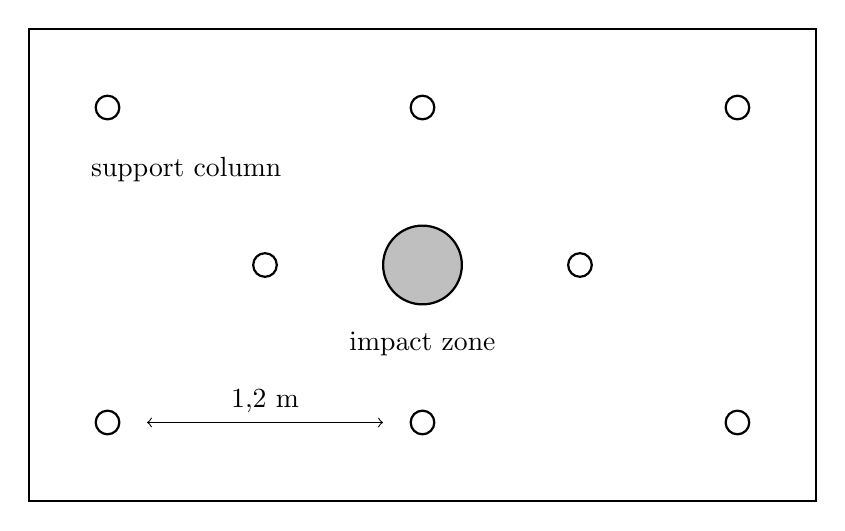
\begin{tikzpicture}
% canadian rock burst drop rig 


\draw[thick] (0,0) -- (10,0) -- (10,6) -- (0,6) -- cycle;
\draw[thick] (1,1) circle [radius=0.15] % pressure points
(5,1) circle [radius=0.15] 
(9,1) circle [radius=0.15] 
(3,3) circle [radius=0.15] 
(7,3) circle [radius=0.15] 
(1,5) circle [radius=0.15] 
(2,4.5) node[align=left, below] {support column}
(5,5) circle [radius=0.15] 
(9,5) circle [radius=0.15];
%[thick] (4.5,2.5)  rectangle (5.5,3.5)
\draw[thick, fill=lightgray] (5,3) circle [radius=0.5];
\draw (5,2) node[align=center] {impact zone}
(3,1) node[align=center,above] {1,2 m};
\draw [<->] (1.5,1) --+ (3,0);
\end{tikzpicture}

\caption{Impact test setup as described by \\ \textcite{canada96}}
\label{fig:can}
\end{figure}

\Textcite[4.24]{canada96} conducted so called "impact tests". 
The experiments were set up in the following fashion:

A weight of 565 kg was dropped on reinforced shotcrete panels measuring 1,5 x 2,75 m, supported on 8 points by dummy bolts, each fitted with a loading cell. The bolts were laid out in a 1,2 x 1,2 diamond pattern.  In \autoref{fig:can} a schematic of the setup is displayed. The maximum drop height was 4 m. The drop weight hit the reinforced shotcrete directly. The drop weight had cylindrical shape, with a diameter of 0,6 m and a hole through the middle for the guidance system.
The results were an approximate linear correlation between impact energy and deformation, with the panels being able to absorb about 15 \(\frac{\text{kJ}}{\text{m}^2}\) and still being functional as static support afterwards.

\section{GAP 611}

\begin{figure}
    \centering
    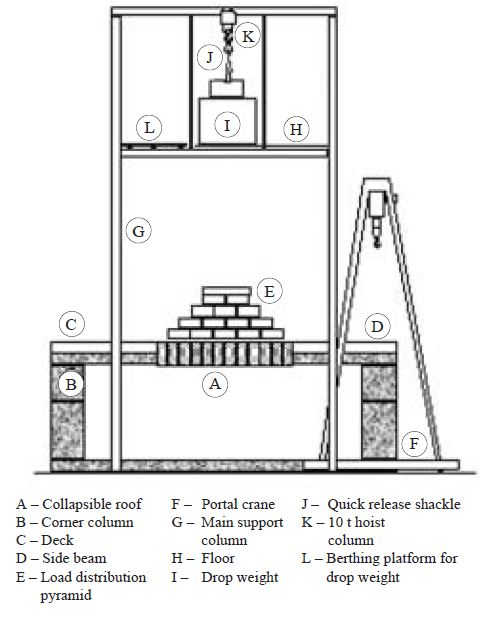
\includegraphics{pics/GAP611_side.JPG}
    \caption{Sideview of GAP611 after \autocite{human04}}
    \label{fig:gap611}
\end{figure}

This facility was built by SIMRAC in 1999 in South Africa. The general set up is displayed in \autoref{fig:gap611}.
The testable area of support is 3 x 3 m. Concrete blocks are placed on the support which simulated the hanging wall. They can move independently of each other. The drop weights hits the simulated hanging wall and the energy is transferred to the support system. \autocite{human04}


\section{GAP 616}

This rig was originally built by SRK consulting and was modified by the Safety in Mines Research Advisory Committee to be able to test more than FRS. The rock mass is represented by concrete bricks. The reason being, that the failure plane between the brick would be vertical. The drops were repeated at the same energy level and height until failure of the system. The concrete was sprayed directly on one layer of the bricks. 


\section{West Australian School of Mines}

\begin{figure}
    \centering
    
\subcaptionbox{Test rig for dynamic tests on bolts\label{fig:WASMbolt}}{
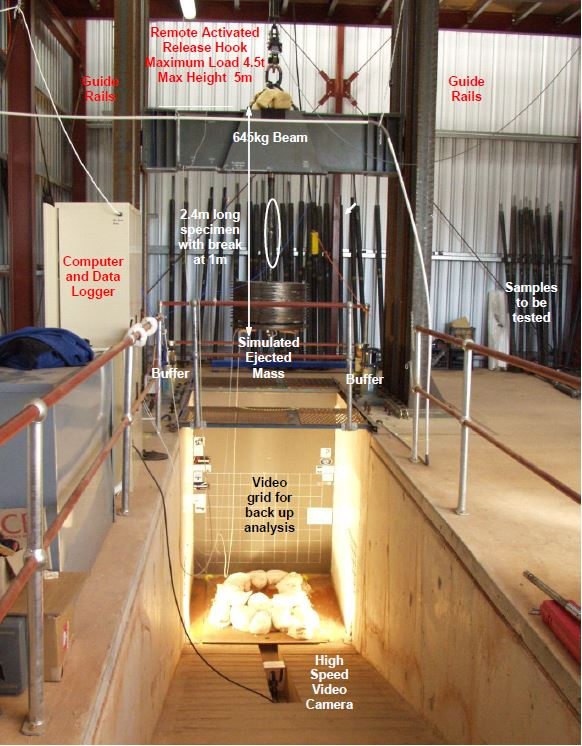
\includegraphics[width=0.45 \linewidth]{pics/WASMbolt.JPG}
}
\subcaptionbox{Test rig for static testing of mesh \label{fig:WASMstatmesh}}{
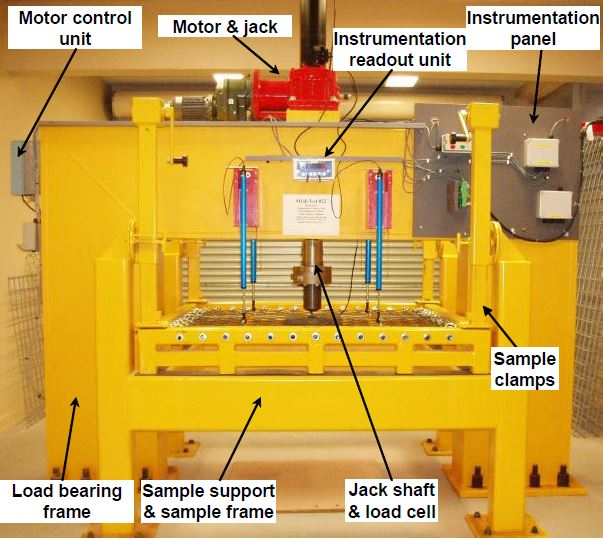
\includegraphics[width=0.45 \linewidth]{pics/WASMstatic.JPG}
}
\subcaptionbox{Test rig for dynamic tests of mesh, note the variable boundary conditions \label{fig:WASMdynmesh}}{
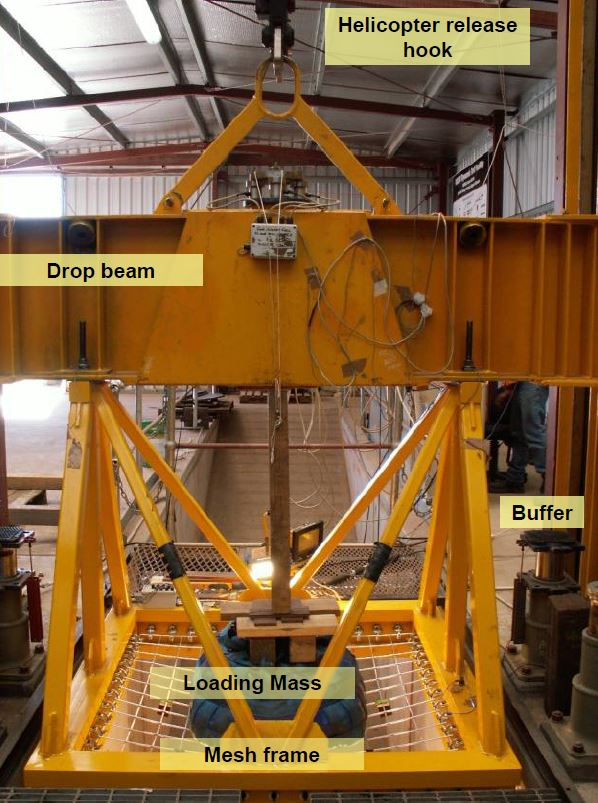
\includegraphics[width = 0.45 \linewidth]{pics/WASMmesh}
}

\caption{Tests rigs built by WASM after \textcite{villa09}}
\end{figure}

The Western Australian School of Mines (WASM) built several dynamic and static testing facilities for testing ground support. The drop test facility uses a different way of transferring load. Instead of dropping a weight on the static support, the support elements and weight are dropped together and slowed by buffers and the energy is transferred during that deceleration. It´s called momentum transfer and is supposed to more closely resemble \textit{in - situ} conditions. Most of their facilities were built in 2004. They built a drop tests rig for bolts (see \autoref{fig:WASMbolt}) a static test rig for mesh, with an very elegant solution to the boundary conditions problem (see \autoref{fig:WASMstatmesh}) a dynamic rig for mesh and concrete panels (see \autoref{fig:WASMdynmesh}).
%As of now it is not possible to test concrete samples with any of their rigs.

\section{NIOSH}

\textcite{Raffaldi17} described the test facilities built by 
the National Institute for Occupational Safety and Health Spokane Mining Research
Division in Spokane, Washington, United States of America. It is a quasi-static and a dynamic testing facility for ground support. The dynamic facility utilises momentum transfer. Only concrete samples can be tested. Mesh can only be used as reinforcement. One type of TSL has been tested. 



%TO DO more test methods!

%\subsubsection{Drop Test}


Building on these machines and the results of their drop tests a drop test rig was developed at Kiirunvaara mine. It was designed with the needs of the mine in mind.